\chapter{Subitizing Systems} 

\label{Chapter 4}
\lhead{Chapter 4. \emph{Subitizing systems}}
\vspace{3cm}
\newpage

\section{Chapter Overview}
% Premise
Whether we realise it or not, many everyday comparisons of quantity occur within the subitizing range, 1--4. For example, when we choose the fewer of two coffee queues, we may rapidly subitize each queue before deciding which one to join. As we go to pay, we might empty our wallet of coins and subitize the gold coins from amongst the silver shrapnel. In both of these instances, we are using a subitizing system to evaluate item-sets when those sets are physically separate (e.g., coffee queues) or intermixed (e.g., coins). But under what processing architecture and workload capacity does this subitizing system operate?

In Chapter 3, we found that two item-sets may be estimated at the same time through a parallel estimation system. As speculated by \citeA{HALBERDA_2006}, subitizing systems may also operate under a parallel processing architecture. In the current Chapter, we aim to address this question of processing architecture with empirical data. Using SFT, we will assess the processing architecture of subitizing systems and determine whether subitizing systems operate under a serial or parallel processing architecture.

In the previous Chapter, we found that estimation systems perform under severe constraints to workload capacity. These constraints were such that the observed parallel processing system was less efficient than that of a theoretical serial processing system. In our discussion of estimation system workload, we noted that the number of items in both item sub-sets may influence the capacity of the system. If true, we should expect workload capacity to be less-limited in a subitizing system, than in the previously measured estimation system. 

An alternative explanation suggests that context effects created the severe limitations in estimate system workload capacity. If the presence of an additional item-set violates the assumption of context invariance --- that the presence of one item-set impacts the processing of the other --- we might expect to see similar limitations in workload capacity between subitizing and estimating systems. If so, we should expect subitizing systems to display severe limitations to workload capacity, with the capacity coefficient measuring at or below the Grice lower-bound. 

In this Chapter, we will characterize information-processing approaches for subitizing two colored item-sets (red and blue discs), when comparing these sets to an internal representation of quantity (three or four items). We will develop an extended double-factorial paradigm using quantities within the subitizing range (1--4). Using experimental data, we will apply the machinery of SFT and assess system workload capacity and processing architecture i) when two item-sets are intermixed and ii) when two item-sets are physically separated. By comparing workload capacity between estimation and subitizing systems, we will determine whether system capacity is impacted by i) the number of items in both item sub-sets, or ii) context effects occurring in the presence of an additional item-set. To foreshadow the results of this study, we find subitizing systems operate under severely limited workload capacity and under predominantly serial processing system architectures.


\section{Subitizing processing architecture}
In the earliest academic account of subitizing, \citeA{jevons1871power} described how five or fewer beans might be counted ``at a glance" without cost to accuracy. Later, \citeA{kaufman1949subtizing} coined the term `subitizing', and showed the time to count four or fewer items was comparable, yet the time to count further items increased with set-size. This led \citeA{kaufman1949subtizing} to speculate that subitizing was a holistic process, capable of quantifying an entire item-set simultaneously. Later, \citeA{pylyshyn1988tracking} extended this account with a visual indexing theory, suggesting a pre-attentive visual tracking system limited to four or fewer items. While more recent work has shown subitizing requires attention \cite{Burr2010}, the notion of a parallel indexing system has remained. Today, subitizing is thought to form part of the Object Tracking System \cite<OTS; also known as the parallel individuation system; >{Hyde2011}, and have a four item-limit due to limitations within visual working memory \cite{cowan2001magical, leslie1998indexing}. 

The ability to subitize a group of items through the OTS, affords the potential of a parallel subitizing system. In their description of `groupitizing', \citeA{starkey2014groupitizing} described how an item-set could be enumerated faster, if the items were grouped into subitizable sets. For example, twelve items may be enumerated faster when grouped into three groups of four, or four groups of three. A speed advantage may be observed when groupitizing for one of two reasons.

Groupitizing might reflect the ability to quickly subitize item sub-sets in sequence, and sum or multiply their value by the number of sub-sets. This strategy could be characterized by a serial processing architecture. Alternately, groupitizing might reflect the ability to subitize the value of multiple item sub-sets at the same time. This strategy could be characterized by a parallel processing architecture. Both parallel and serial subitizing systems would predict faster enumeration than the serial counting of each item individually. Diagnosing whether subitizing systems operate in parallel or serial is one aim of the current study. 

\subsection{Subitizing workload capacity}
As previously noted, workload capacity will form an important line of investigation within the current study. In the previous Chapter, we found severely limited workload capacity within parallel estimation systems. This limitation was either due to i) the number of total items in the stimulus array, or ii) the violation of context invariance where the enumeration of one item-set was impaired by the presence of another. If the number of displayed items altered workload capacity, we expect capacity coefficient results to be less-limited in the current investigation. However, if workload was limited due to context effects, we expect workload capacity results to mimic those of the previous Chapter. Specifically, we expect workload capacity to be limited to such a degree, that the capacity coefficient violates the Grice lower-bound. With clear expectations for processing architecture and workload capacity in place, we must now consider the design and quantities that will be used in the current study. 

\subsection{Subitizing targets and distractors}
In Chapter 2, we performed a pilot study to select target and distractor quantities within the range of estimation for use in an expanded double-factorial paradigm. The primary aims of this study were to i) select target quantities that would result in a numerical distance effect on RT, and ii) ensure accurate responses. In the current study, we aim to use an extended double-factorial paradigm to test systems of subitizing. Therefore, targets quantities must be within the range of 1--4. As a result, we expect all responses to be highly accurate as subitizing is characteristically an accurate process.

In the selection of target quantities, a number of considerations must be made. While the subitizing range is generally considered to range from 1--4, this range has been shown to vary from individual to individual \cite<for example,>{green2003action}. As a conservative measure, we will limit our maximum target value to 3. Having defined our maximum target, we must now define our smallest target. 

A single item may be evaluated by the process of subitizing, or by a process of perceptual detection. In the context of an enumeration task, it is likely a single-item will engage the process of subitizing due to the task-context. However, there is a chance participants will associate the detection of a single-item with a target-response, potentially facilitating response-times. As such, conclusions regarding processing architecture and workload should not be limited to when target items include only a single unit, (\eg 1 vs 2, or 1 vs 3). To address this, we will perform two concurrent investigations. In one investigation, we will adopt a criterion of three items; targets will be one-item and two-items. For symmetry to the target sets, distractors will be four-items and five-items. In the second investigation the criterion will be four-items; targets will be two-items and three-items, and distractors will be five-items and six-items. 

Similar to our investigation of estimation systems, we must consider the effect of low-level perceptual covariates on the subitizing system. For this reason, each investigation will control for the effect of item-set area in a similar manner to Chapter 3. This will be completed in conjunction with the manipulation of item-set separation (intermixed vs separate color-sets), within the framework of an extended double-factorial design.


\section{Method}
The method of this study is very similar to that of the previous chapter. For the sake of brevity, only the primary differences will be described. The first factor manipulation of our expanded double-factorial paradigm was the presence or absence of a target item-set. Target-sets were defined as containing fewer than either a criterion of three or four items. Distractor-sets were defined as containing more than the criterion. 

At the second factor level, the salience of each item-set was manipulated relative to the central criterion of three or four items. Salience was manipulated through the numerical distance effect \cite{buckley1974comparisons}; quantities closer to the criterion were harder to evaluate than quantities further away. High-salience targets were defined as being two items fewer than the criterion and low-salience targets were defined as being one item fewer than the criterion. High-salience distractors contained two more items than the criterion and low-salience distractors contained one more item than the criterion.

As in Chapter 3, we applied an expanded double-factorial design across four experiments to assess the impact of spatial separation and low-level perceptual covariates on the subitizing system. Figure \ref{fig:subStim} illustrates the experimental stimuli for a criterion of three, and how they differed across the four factorial manipulations of item-set area and item-set separability (left-to-right, experimental manipulations 1--4; Figure \ref{fig:subStim}).

%The first experimental manipulation assessed subitizing systems when two colored item-sets were intermixed. The second manipulation assessed subitizing systems when item-sets were physically separated. The third manipulation assessed subitizing systems when item-sets were intermixed and item-set area was matched. The final manipulation assessed subitizing systems when item-sets were separated and item-set area was matched.


\begin{figure}[hbt]
\centering \includegraphics[width=\linewidth]{Figures/Subitizing/SubStim.jpg}
\caption{Example stimuli using a criterion less-than three, when discs were of a fixed size (left), and when item-set area was fixed (right); for mixed and separate item-set designs. Each example illustrates a conflict-target response-condition, where one color-set is fewer than three, and one color-set is greater than three.}
\label{fig:subStim}
\end{figure}


\subsection{Participants}
Participants were undergraduate psychology students from the University of Newcastle, Australia, who completed a 90 minute experiment for three course-credits. All participants reported  normal or corrected to normal vision, and intact color vision. The number and mean age of participants in each experiment are displayed in Table \ref{tab:Sub_Participants}.

\begin{table}[htb]
\centering
\caption{Participant number and mean age, for each experiment.}
\begin{tabular}{l l l l l l} 
\hline
Exp & Criterion & \begin{tabular}{l} Perceptual \\ Control \end{tabular} & \begin{tabular}{l} Item-Set \\ Proximity \end{tabular} & \begin{tabular}{l} Participants \\ (Female) \end{tabular}  & Age (SD) \\
\hline
1.1 & 3 &~Fixed Disc Size   &~Mixed     &~9 (5) & 22.67 (8.59) \\
1.2 & 3 &~Fixed Disc Size   &~Separate  &~6 (4) & 26.5 (14.63) \\
1.3 & 3 &~Matched Set Area  &~Mixed     &~9 (6) & 22.67 (6.08) \\
1.4 & 3 &~Matched Set Area  &~Separate  &~5 (3) & 22.6 (2.07) \\
\hline
2.1 & 4 &~Fixed Disc Size   &~Mixed     &~8 (4) & 22 (3.3)  \\
2.2 &4 &~Fixed Disc Size   &~Separate  &~10 (6) & 20 (1.87) \\
2.3 &4 &~Matched Set Area  &~Mixed     &~8 (6) & 24 (5.04)  \\
2.4 &4 &~Matched Set Area  &~Separate  &~8 (5) & 23.89 (5.58)  \\
\hline
\hline
\label{tab:Sub_Participants}
\end{tabular} 
\end{table}

\subsection{Stimuli and apparatus}
The testing facilities and stimulus properties, (e.g., color, presentation), were identical to those used in Chapter 3. In the first experimental manipulation, the size of each disc was fixed and item-sets were intermixed. In the second experimental manipulation, the size of each disc was fixed, however, item-sets were confined to the top or bottom hemisphere of the central circular field-of-view. In the third experimental manipulation, item-sets were intermixed, and the size (radius) of each item varied. On each trial, the \textit{total} areas of the red and blue color-sets were matched. Color-set area was randomly sampled at the start of each trial and varied within a range of 74-222 pixels, and 98--294 pixels, for criterion three and four respectively. The final experimental manipulation matched item-set area (as previously described), and presented item-sets in either the top or bottom hemispheres of the central circular field-of-view (see Figure \ref{fig:subStim}). 

\subsection{Procedure}
The procedure of this experiment matched that of the previous Chapter, with the addition that participants were randomly allocated to either a criterion three or criterion four task, and to one of the four factorial manipulations of item-set area and item-set separability. 

% Each participant completed a single 90 minute experimental session and were randomly allocated to a criterion 3 or criterion 4 task. Participants were presented with an information sheet and consent form, and answered demographic questions regarding age, gender, handedness, vision and color-blindness. Participants were asked to complete a redundant-target subitizing task, in which any display containing a target set (number of discs in set $<$ 3 or $<$ 4, depending on allocation) called for a `yes', target-present response. Any display containing only distractor item-sets (e.g., a double-distractor or a single-distractor only item-set), called for a `no', target-absent response. Participants responded `yes' to the presence of a target with the `z' key and `no' to the absence of a target with the `/' key. Response keys were counter-balanced across participants.

% At the start of each trial, participants were directed to look at a central fixation cross, presented for 500ms and followed by a 500ms blank screen. The stimulus display was then presented for 500ms, followed by a mask for 500ms and a post-mask blank for 3000ms. From the onset of the stimulus, participants had 4000ms to make a response. The trial ended when the participant made a response or the trial timed-out at the conclusion of the response window. Note that a 500ms stimulus display was used in this task. Subitizing is a rapid enumeration process, and a longer display time might encourage participants to count, rather than subitize each item-set.

% Participants completed one practice block and 15 experimental blocks, each containing 96 randomly ordered trials. Trial-by-trial accuracy feedback was provided during the practice block. Each block contained 12 double-target trials, 12 double-distractor trials, 24 conflict-target trials, 24 single-target trials and 24 single-distractor trials, presented in a random order. These trials were evenly distributed among the constituent salience levels. For example, three trials were presented from each double-target salience combination --- 12 in total. By comparison, six trials were presented from each of the red and the blue, single-target high and single-target low salience conditions --- 24 in total. Not including practice trials, each subject completed 180 double-target trials, 180 double-distractor trials, 360 conflict-target trials (180 target-red, 180 target-blue), 360 single-target trials (180 target-red, 180 target-blue) and 360 single-distractor trials (180 distractor-red, 180 distractor-blue). In total, subjects completed 1440 experimental trials with a 5:3 yes/no response bias. The probability of a target item-set in one color (e.g., red), given a target item-set in the other color (e.g., blue), was 0.33 \cite{mordkoff1991}.

\section{Data analysis}
Incorrect trials, and trials with response times less than 150 ms or greater than the 97.5$^{th}$ percentile were excluded from analysis. Participants' data were included if their total accuracy was $>80\%$ correct, \emph{and} their conditional accuracy in each of the six target conditions was $>66\%$. All repeated-measures ANOVAs were corrected for violations of sphericity, where appropriate, using the Greenhouse-Geisser correction. Post-hoc paired $t$-tests were corrected for family wise error using the Bonferroni method. As in the previous Chapter, workload capacity was assessed through the redundant target effect \cite<RTE; >{miller1982divided, eidels2008similarity}, capacity coefficient and resilience difference function. Processing architecture was assessed for double-target conditions using the MIC and SIC($t$). Selective influence between the double-target salience conditions was assessed for each subject using a series of non-parametric KS tests at an alpha $p <$ .15 \cite{johnson2010systems}. 

\color{\Red}
\section{Results}
\subsection{Accuracy}
Participants with conditional accuracy $< 66\%$ or total accuracy $< 80\%$ were excluded from analysis. Thirteen participants were excluded across all experiments, displayed separately for each experiment in Table \ref{tab:Sub_Acc}. Accuracy was high for the remaining participants across experiments ($M$ = .91, $SD$ = 0.04). The rest of the analysis will focus exclusively on assessments of response-time.

\begin{table}[htb]
\centering
\caption{Participant exclusions and mean accuracy in each experiment.}
\begin{tabular}{ l l l l l l } 
\hline
Exp & Criterion & 
\begin{tabular}{l}Perceptual \\Control \end{tabular} & \begin{tabular}{l}Item-Set \\Proximity \end{tabular} & Excluded N & \begin{tabular}{l}Mean \\Accuracy (SD) \end{tabular} \\
\hline
1.1 & 3 &~Fixed Disc Size   &~Mixed     & 1  &~.92 (.05) \\
1.2 & 3 &~Fixed Disc Size   &~Separate  & 0  &~.94 (.02) \\
1.3 & 3 &~Matched Set Area  &~Mixed     & 1  &~.92 (.05) \\
1.4 & 3 &~Matched Set Area  &~Separate  & 1  &~.90 (.06) \\
\hline
2.1 & 4 &~Fixed Disc Size   &~Mixed     & 3 &~.90 (.02)  \\
2.2 & 4 &~Fixed Disc Size   &~Separate  & 2 &~.89 (.01) \\
2.3 & 4 &~Matched Set Area  &~Mixed     & 4 &~.92 (.03)  \\
2.4 & 4 &~Matched Set Area  &~Separate  & 1 &~.90 (.05)  \\
\hline
\hline
\label{tab:Sub_Acc}
\end{tabular} 
\end{table}

\subsection{Target mean RT}
The following section focuses on %AE: focuses ON,  not UPON (though grammatically correct)
our conditions of load: the double-target (Dt), red single-target (Rt), and blue single-target (Bt) conditions. These response-sets are formed from the combination of their nested salience levels. For example, red single-target responses are the aggregate pool of all high (H) and low (L) red target-salience trials, and double-target responses include combinations of HH, HL, LH and LL red-and-blue target-salience levels.

Mean response-time (mRT) results for all experiments are plotted in Figure \ref{fig:subMeanRT}. In each experimental manipulation, regardless of criterion, double-target responses tended to be slower than either single-target red or single-target blue responses. Comparing single- vs double-target conditions, there was a significant effect of workload (number of targets) on response-time, summarized in Table \ref{tab:Sub_ANOVA}. Paired sample $t$-tests were conducted to explore these differences further (fully reported in the supplementary materials, Table \ref{tab:Sub_ttests}). 

%AE: paul, you have used the term 'within target-conditions ' a couple of times above, which i have found a bit confusing, and replaced. consider my suggestion and implement for the rest of the text if you see fit

As seen in Figure \ref{fig:subMeanRT}, double-target responses were significantly slower ($p <$ .05) than at-least-one single-target response condition, in all except two experimental manipulations. There was no significant response-time difference between single- vs double-target conditions when the criterion was three, item-set area was fixed and item-sets were separated. Similarly, here was no significant response-time difference between single- vs double-target conditions when the criterion was four, item-size was fixed, and item-sets were intermixed. No significant response-time differences were observed between red and blue single-target responses, regardless of criterion or experimental manipulation. Overall, these results suggest participants experienced a \textit{redundancy cost} when subitizing two target item-sets. For further insight, we also consider the effects of redundant targets at the individual level.

\begin{figure}[hbt]
\centering \includegraphics[width=\linewidth]{Figures/Subitizing/MeanRTsig.jpg}
\caption{Mean response-time for double-target (Dt), red single-target (Rt) and blue single-target (Bt) conditions, when the criterion was three (top) or four (bottom), and when item-size was fixed (left), and when item-set area was fixed (right). Black markers indicate mixed item-set conditions, white markers indicate separated item-set conditions. Error bars indicate the standard error of the mean. Bonferroni corrected, paired $t$-test significance: * $p <$ .05, * $p <$ .01, * $p <$ .001. }
\label{fig:subMeanRT}
\end{figure}

\begin{table}[htb]
\centering
\caption{Repeated-measures ANOVA results for assessments of target workload in each experiment.}
\begin{tabular}{ l l l l l} 
\hline
Exp & Description & $F$ (df) & Sig & $\eta_{p}^{2}$ \\
\hline
1.1 & Crit 3; Fixed Size; Mixed & 14.93 (2,14)  & $<$ .001 & 0.68  \\
1.2 & Crit 3; Fixed Size; Separate & 5.846 (2,10)  & $<$ .05 & 0.54\\
1.3 & Crit 3; Fixed Area; Mixed & 20.67 (2,14)  & $<$ .001 & 0.75 \\
1.4 & Crit 3; Fixed Area; Separate & 5.353 (2,6)  & $<$ .05 & 0.64 \\
\hline
2.1 & Crit 4; Fixed Size; Mixed & 11.57 (2,8)  & $<$ .01 & 0.74  \\
2.2 & Crit 4; Fixed Size; Separate & 102.9 (2,14)  & $<$ .001 & 0.94\\
2.3 & Crit 4; Fixed Area; Mixed & 59.14 (2,6)  & $<$ .001 & 0.95 \\
2.4 & Crit 4; Fixed Area; Separate & 44.26 (2,7.8)$^+$  & $<$ .001 & 0.86 \\
\hline
\hline
\multicolumn{4}{l}{$^+$ Greenhouse geisser corrected.}
\label{tab:Sub_ANOVA}
\end{tabular} 
\end{table}

\subsection{Redundant target effect}
Figure \ref{fig:subRTE} displays the mean redundant target costs for each subject, broken down by criterion and experimental manipulation. As shown, every participant experienced a redundancy cost (negative RTE), regardless of criterion or manipulation. All individual redundancy costs were significant, measured at the distributional level using a KS alpha $<$ .15. This suggests the addition of a second target slows the subitizing-system, a hallmark of limited capacity processing.


\begin{figure}[hbt]
\centering \includegraphics[width=\linewidth]{Figures/Subitizing/RTE.jpeg}
\caption{Redundant target costs, displayed as separate markers for each individual. All redundancy costs were significant at the distributional level, KS alpha $<$ .15.}
\label{fig:subRTE}
\end{figure}

Redundancy costs were, on average, greater when the criterion was four than when it was three. This may indicate i) an interaction between workload and criteria, ii) a simple effect of criteria on workload, or iii) a proportional increase across all RTs for the criterion four conditions, (\ie a global redundancy cost caused by an overall increase in RT).

To assess whether redundancy costs changed differentially, (\ie interacted), with criteria, several two-way between-subjects ANOVAs were conducted. When item-size was fixed and item-sets were intermixed, there was no main effect of load, (\ie double-target mean RT vs the fastest single-target mean RT; \Fval{1}{22}{4.18}{= 0.05}, $\eta^2$ = 0.16), and no main effect of criteria (\Fval{1}{22}{0.332}{= 0.57}, $\eta^2$ = 0.01). No interaction effect between criteria and load was observed (\Fval{1}{22}{0.474}{= 0.5}, $\eta^2$ = 0.02). Similarly, when item-size was fixed and item-sets were separate, there was no effect of load (\Fval{1}{24}{4.209}{= 0.05}, $\eta^2$ = 0.14), and no effect of criteria (\Fval{1}{24}{0.982}{= 0.33}, $\eta^2$ = 0.03). No interaction effect was observed between criteria and load (\Fval{1}{24}{0.559}{= 0.46}, $\eta^2$ = 0.02). 

When area was fixed and item-sets were mixed, there was a main effect of load (\Fval{1}{20}{6.941}{$<$ 0.05}, $\eta^2$ = 0.2), and a main effect of criteria (\Fval{1}{20}{7.236}{$<$ 0.05}, $\eta^2$ = 0.2). No interaction effect was observed between criteria and load (\Fval{1}{20}{1.377}{= 0.25}, $\eta^2$ = 0.04). Finally, when area was fixed and item-sets were separate, there was no main effect of load (\Fval{1}{20}{1.692}{= 0.21}, $\eta^2$ = 0.05), and a main effect of criteria (\Fval{1}{20}{11.313}{$<$ 0.01}, $\eta^2$ = 0.34). No interaction effect was observed between criteria and load (\Fval{1}{20}{0.166}{= 0.68}, $\eta^2$ = 0.01).

Independent samples $t$-tests were conducted to assess the effect of criteria on the redundancy cost. When item-size was fixed and item-sets were mixed, redundancy costs did not significantly differ between criteria three (M = -49ms, SD = 25ms) and four (M = -97ms, SD = 58ms; \tval{-.679}{10}{= .51}). When item-size was fixed and item-sets were separate, redundancy costs significantly increased from criterion three (M = -37ms, SD = 11ms) to four (M = -78ms, SD = 15ms; \tval{2.559}{9}{$<$ .05}).

When area was fixed and item-sets were mixed, redundancy costs significantly increased from criterion three (M = -29ms, SD = 12ms) to four (M = -75, SD = 12ms; \tval{7.199}{14}{$<$ .001}). Finally, when area was fixed and item-sets were separate, redundancy costs significantly increased from criterion three (M = -39ms, SD = 18ms) to four (M = -74ms, SD = 25ms; \tval{3.388}{6}{$<$ .05}).

Finally, to assess whether the observed increase in redundancy costs were due to an overall proportional increase in RT between criterion three and four trials, we replicated the above analysis with log$_{10}$ transformed response-times. All of the above effects held with log RT, indicating the effects were not caused by an overall or proportional increase in RT between the criteria. 

%%AE1: < sign does not seem to compile properly. AE2: the above section is a bit much, dot you think it is a tad long? in any event, leave it as is for now, not worth investing time to modify...
Results from the RTE and redundancy cost analyses indicate that workload significantly increased with criteria in three of the four manipulations. This effect was not explained by a global increase in response-times, or an interaction effect of response-time and load. It might be that a different cognitive process is occurring when the criterion was three, as to when the criterion was four. The nature of this process is yet unclear. %AE: discard >>These results are interesting and provide a clear comparison between criteria at the level of the mean. 
For further interpretation of individual subject's workload capacity over the entire response-time range, we now turn to the capacity coefficient analysis.

\subsection{Capacity coefficient}
The capacity coefficient allows clear interpretation of performance limitations, compared to an established benchmark UCIP model. Figure \ref{fig:subCap} displays group mean and individual capacity coefficient [C($t$)] results, for each criterion, and each experimental manipulation. In line with the previous redundancy costs, capacity coefficients display limited workload capacity, C($t$) $<$ 1, at both the group (black line) and individual (grey markers) level. Furthermore, each plot depicts \Ct hovering below the Grice lower-bound (broken line) for most of the response-time range\footnote{Late or early crossings of the Grice lower-bound do not reflect a sudden change in workload capacity. Rather, this indicates where the response-time range is poorly defined, (\ie where there are too few double-target responses to make a stable estimate.)}. Individual low-bounds present at approximately \Ct = 0.5, with all individual \Ct scores resting at or below the low-bound for the majority of the response-time range (individual \Ct plots for each experiment can be found in the supplementary materials, Figure \ref{fig:AppB_subCap1} -- Figure \ref{fig:AppB_subCap4}). These results suggest most individuals experienced severe capacity limitations when estimating multiple item-sets.

Analysis of the capacity coefficient and RTE show all subjects subitized multiple target-sets with limited workload capacity. Furthermore, performance of most subjects was below the Grice lower-bound, suggesting they experienced limitations typically associated with a serial processing system. Interpretation of processing architecture and workload capacity, can be extended with our next measure, the resilience difference function. 

\begin{figure}[hbt]
\centering \includegraphics[width=\linewidth]{Figures/Subitizing/SubCapacity.jpeg}
\caption{Capacity coefficient (C($t$)) plots for target-present responses. Group mean \Ct is plotted in black with the Grice lower-bound, an estimate of severe capacity limitations, depicted by the dashed line. Individual participant \Ct values are illustrated by gray markers and mostly fall at or below the group Grice bound, indicating severe capacity limitations across all experimental manipulations.}
\label{fig:subCap}
\end{figure}

\subsection{Resilience difference function}
Resilience difference (R$_{diff}$($t$)) values for the group mean as well as individual subjects, for high target-salience trials, are plotted in Figure \ref{fig:subRdiffHigh}. Interpretation of these results can be aided by comparison to \Rd predictions, presented previously in Figure \ref{fig:Rd}. In all cases, \Rd hovers around zero, for most of the response-time range. While these \Rd functions are far less stable than those observed within the range of estimation, in general, these findings align with the predictions of a parallel minimum-time unlimited-capacity processing system (\Rd = 0). Similar results were displayed by \Rd functions when target salience was low (see Figure \ref{fig:subRdifflow}). While \Rd provides some insight into processing architecture for conflict-target conditions, further interpretation of target architecture requires analysis of the mean and survivor interaction contrasts.

\begin{figure}[hbt]
\centering \includegraphics[width=\linewidth]{Figures/Subitizing/SubRdiffHigh.jpeg}
\caption{Resilience difference plots for when target salience was high and the criterion was three or four, for each experimental manipulation. Black lines depict the average resilience difference function across subjects, while grey markers illustrate individual subject’s resilience difference functions. Average plots show a trend towards \Rd = 0, supporting predictions made by an unlimited-capacity parallel minimum-time processing system.}
\label{fig:subRdiffHigh}
\end{figure}

\begin{figure}[hbt]
\centering \includegraphics[width=\linewidth]{Figures/Subitizing/SubRdiffLow.jpeg}
\caption{Resilience difference plots for when target salience was low and the criterion was three or four, for each experimental manipulation. Black lines depict the average resilience difference function across subjects, while grey markers illustrate individual subject’s resilience difference functions. Average plots show a trend towards \Rd = 0, supporting predictions made by an unlimited-capacity parallel minimum-time processing system.}
\label{fig:subRdifflow}
\end{figure}

\subsection{Double-target processing architecture}
In the following section, we will report the MIC and SIC, as calculated from the response-time differences between double-target salience manipulations --- high-high (HH), high-low (HL), low-high (LH) and low-low (LL). Valid interpretation of the mean interaction contrast (MIC) requires two basic assumptions. The MIC requires selective influence, which is often gauged empirically via the successful manipulation of salience within both target color-sets (determined by the main effects of a between-subjects ANOVA), and correct ordering of the salience conditions, (\ie mRT$_{HH}$ $\leq$ mRT$_{HL}$, mRT$_{LH}$ $\leq$ mRT$_{LL}$). For the MIC, a statistical interaction between the salience levels of each color-set acts as a test for parallel processing architectures, and thus will also be reported. The SIC($t$), in addition to the previous assumptions, requires the assumption of selective influence to hold at the level of the survivor functions, (\ie S($t$)$_{HH}$ $\leq$ S($t$)$_{HL}$, S($t$)$_{LH}$ $\leq$ S($t$)$_{LL}$). Reported MIC and SIC results are limited to those subjects who met the necessary criteria for valid interpretation. 

%AE: above, sign should be equal or smaller than (not just smaller than) -- same fr SIC below. Also, the actual assumption is selective influence, the salience effects and ordering are the empirical test
% PG: Thanks for catching this! 

In the previous Chapter, we classified participant processing architecture using the newly developed non-parametric Bayesian SIC assessment technique, provided by \citeA{houpt2017bayesSIC}. Across all tested participants, only ten met the necessary assumptions for SIC analysis; however, many participants met the assumptions for MIC analysis. As such, results focus on %AE: c'ommon -- upon 
the MIC, and were applicable, are supplemented by SIC interpretations. As in the previous Chapter, processing architecture classification was aided by the hierarchical Bayesian MIC analysis, developed by \citeA{houpt2017hierarchical}. This analysis takes into account data across all valid participants in each experiment. We enhance these results with classical MIC and SIC diagnostic techniques, including visual inspection of individual MIC and SIC plots, and statistical tests for parallel processing architectures. For clarity of exposition, we first summarize the results of classified subjects across all experiments, then present a breakdown by individual subjects. 

\subsubsection{Summary of architectures}
The left panel of Figure \ref{fig:subArchSummary} shows the range of MIC values for subjects who met SIC and MIC inclusion criteria in each experimental type, collapsed across criteria. The majority of subjects in each experiment recorded a positive MIC value, supporting parallel minimum-time processing architectures. Yet, error bars extend to the zero MIC and median MIC values hover near zero, allowing the possibility of serial processing systems. The right panel of Figure \ref{fig:subArchSummary} shows the proportion of processing architectures in each experiment, after classification. Classification reflects the combination of visual and statistical inspection of the MIC and SIC, and hierarchical Bayesian MIC analysis. Each bar represents the total number of classified subjects in each experiment (N reported below each bar), with the shaded regions marking the relative proportion of subjects based on the way they enumerate two target sets (in parallel or serial). When item-set area was fixed and item-sets were separated, the majority of participants displayed a parallel processing architecture. In all other experimental conditions, the majority of subjects displayed serial processing architectures. For simplicity, summary results were collapsed to the serial and parallel categories, across minimum-time and maximum-time stopping-rules. The next section presents individual processing architecture and stopping-rule results. 

\begin{figure}[hbt]
\centering 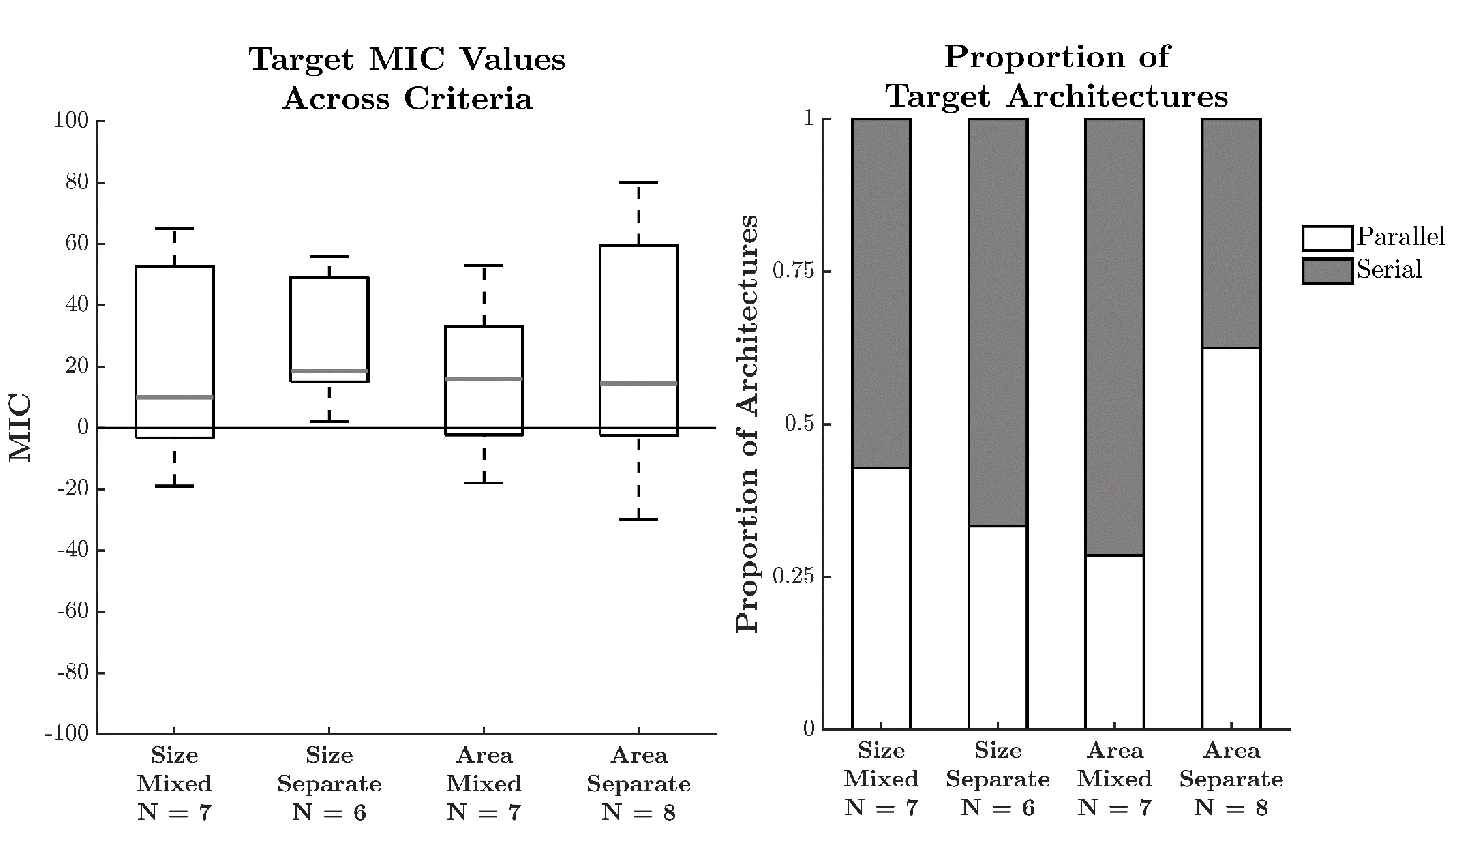
\includegraphics[width=\linewidth]{Figures/Subitizing/ArchSummary3v2.pdf}
\caption{MIC values (left) and the proportion of categorized processing architectures (right) collapsed across criteria. Proportions are relative to the total number of subjects who could be classified using MIC and SIC significance testing. For simplicity, classified architectures have been displayed without stopping-rule.}
\label{fig:subArchSummary}
\end{figure}

\subsubsection{MIC plots}
In the previous Chapter, we noted that the classification of processing architecture can be aided by interpretation of MIC plots. Figure \ref{fig:subMIC1} displays the MIC plots for three participants, when the criterion was less-than three, item-size was fixed and item-sets were mixed. Within ecah panel, each marker denotes a combination of red-target and blue-target salience --- HH, HL, LH and LL. Focusing on %upon 
participant SM 304 (left panel), the MIC value is not significantly different than zero, mean RTs are ordered appropriately, and no interaction of high and low target-salience is apparent in the plot (denoted by the parallel lines and no significant ANOVA interaction). Participant SM 306 follows a similar account; both subjects display results consistent with a serial processing architecture. By contrast, participant SM 308 shows a negative MIC value (-19) with a significant, under-additive interaction term. This interaction is consistent with a parallel exhaustive (maximum-time) processing architecture. Remaining MIC plots for each participant may be found in supplementary materials, Figure \ref{fig:AppB_MIC1} and Figure \ref{fig:AppB_MIC2}. We will summarize these results shortly in Table \ref{tab:subArch}. Processing architecture and stopping-rule classification can be further aided by our next analysis tool, the SIC. 

\begin{figure}[hbt]
\centering 
\includegraphics[width=\linewidth]{Figures/Subitizing/SubMIC.jpg}
\caption{Mean interaction contrast plots for three subjects when the criterion was three, item-size was fixed and item-sets were mixed. The left and middle panel display MIC signatures in line with predictions of a serial (additive) processing architecture. The right panel displays an MIC signature in line with an under-additive MIC signature (parallel maximum-time). * denotes a significant ANOVA interaction, a hallmark of parallel processing architectures. Error bars represent $\pm$ one standard-error of the mean.}
\label{fig:subMIC1}
\end{figure}


\subsubsection{SIC plots}
Figure \ref{fig:subSIC} displays individual SIC($t$) plots, for all participants who met the assumptions of selective influence (at KS alpha $<$ .15) required for valid interpretation. To aid SIC($t$) interpretation, each plot has been augmented with statistical tests \cite{houpt2010statSIC} denoting a significant positive (D+) or negative (D-) deviation from a zero SIC. Recall that a parallel minimum-time processing architecture predicts an all positive SIC($t$), a parallel maximum-time processing architecture predicts an all negative SIC($t$), and a serial maximum-time architecture predicts an SIC($t$) that transitions from negative-to-positive with an MIC = 0. 

\begin{figure}[hbt]
\centering \includegraphics[width=\linewidth]{Figures/Subitizing/SubSIC.jpeg}
\caption{Individual participant SIC($t$) functions, across criteria and experimental manipulations. The black line illustrates the SIC($t$) function, and the dashed line $\pm$1 standard error. Significant positive or negative SIC($t$) deviance from zero are denoted by D$\pm$. Significant MIC interaction terms, indicative of a parallel processing system, are denoted by an *. SM - fixed Size, Mixed item-sets; SS - fixed Size, Separate item-sets, AM - fixed Area, Mixed item-sets. Criterion three experiments are further separated by missing planels.}
\label{fig:subSIC}
\end{figure}

%%AE: figure looks a bit odd -- why are there missing panels ?
% PG: It separates Criterion 3 experiments, added to caption.

The previous MIC signatures of participants SM 304, SM 306 and SM 308 were aligned with a serial, serial and parallel minimum-time processing architecture, respectively. The top three panels of Figure \ref{fig:subSIC} display the SIC($t$) of these three subjects. The SIC($t$) signatures of SM 304 and SM 306 transition from negative-to-positive with a negative deviation (D-), typical of a serial maximum-time processing architecture. These signatures do not display a significant positive deviation (D+), yet, given the MIC is near zero and there is no interaction between target-salience, a serial exhaustive processing system is the most plausible classification. Returning now to the parallel maximum-time MIC signature of SM 308. As predicted by a parallel maximum-time processing architecture, SM 308 displays a negative SIC($t$), and significant negative deviation (D-). Finally, as an example of parallel minimum-time processing, consider participant SS 304. SS 304 displays a positive SIC($t$) function with a significant deviation (D+), a positive MIC and significant MIC interaction. These properties fit precisely with predictions of a parallel minimum-time processing system. Using similar classification methods to those described here, processing architectures have been classified using the MIC and SIC for every individual and are summarized in Table \ref{tab:subArch}. To finalize our analysis, we may now consider our last metric, the hierarchical MIC.

\subsubsection{Hierarchical MIC results}
Table \ref{tab:subArch} summarizes the results of all processing architecture analyses, for each participant. From left-to-right, the table displays the participant ID, the MIC value (and interaction significance *), hierarchical MIC Bayes factor values (\textsubscript{H}BF$_{10}$) for the best fitting processing model (\textsubscript{H}MIC), model categorization of the MIC plot, and model categorization of the SIC plot. Group posterior Bayes factors and associated model categorizations are also reported for each experiment\footnote{Hierarchical MIC analysis was also conducted by collapsing across criteria within each experimental manipulation, however, these results were less informative than the results of the presented table. Differences between the response-time distributions of each criterion, in addition to low participant numbers, produced poorer model fits and Bayes factors close to zero for most individuals.}. To interpret the hierarchical MIC Bayes factor results, we follow the classification scheme of \citeA{lee2014bayesian}, adjusted from \citeA[Appendix B]{jeffreys1961theory}. At the individual and group level, Bayes factors for the best fitting processing model tended towards anecdotal evidence (BF$_{10}$ $<$ 3). In these instances, processing model classification was based on the MIC and SIC plots (as previously described). Where Bayes factors provided moderate evidence towards a single processing model (BF$_{10}$ $<$ 5), hierarchical classifications aligned with the MIC and SIC plot classifications. For ease of exposition, the `winning' processing model classification for each participant is displayed in bold font, in the column denoting how processing architecture was best classified. These processing models were used to create the previous summary in Figure \ref{fig:subArchSummary}. Note that the MIC and hierarchical MIC could not identify the stopping-rule of serial processing architectures.

\clearpage
\begin{table}[!htb]
\caption{Table of individual double-target MIC and SIC results across criteria (subject ID 300 vs 400). The winning model categorization for each subject is displayed in bold font. From left to right, participant ID, MIC value and interaction significance (*), Bayes factor values from the hierarchical MIC analysis and associated MIC model (Parallel: P; Serial S), MIC plot model categorization, and SIC plot model categorization. MIC significance tests conducted at * $<$ .33, ** $<$ .05 and *** $<$ .01. Subject ID abbreviations, SM - fixed Size, Mixed sets; SS fixed Size, Separate sets; AM - fixed Area, Mixed sets; AS - fixed Area, Separate sets.}
\centering 
\begin{tabular*}{\textwidth}{l @{\extracolsep{\fill}} rlllll}
\hline
\textbf{Sub  } & \textbf{MIC} & \textbf{\textsubscript{H}BF$_{10}$} & \textbf{\textsubscript{H}MIC Model}  & \textbf{MIC Plot} & \textbf{SIC Plot}\\  
\hline
SM 304  & -6  & 2.23 & Serial & Serial & \textbf{S Max-Time} \\ % S 4.35
SM 306  & 5  & 2.33 & Serial  & Serial & \textbf{S Max-Time} \\ % S 4.34
SM 308  & -19*  & 2.33 & Serial  & P Max-Time & \textbf{P Max-Time} \\ % S 2.57
\multicolumn{2}{r}{Group Posterior} & 1.5 & Serial & ~ & ~\\
\hline
SS 304  & 49*  & 4.32 & P Min-Time  & P Min-Time & \textbf{ P Min-Time} \\ % S 1.3
SS 305  & 15  & 2.9 & P Min-Time  & \textbf{Serial} & \textbf{ - } \\
\multicolumn{2}{r}{Group Posterior} & 2.88 & P Min-Time & ~ & ~ \\
\hline
AM 301  & 9  & 2.13 & Serial  & \textbf{Serial} & \textbf{ - } \\
AM 302  & 16  & 1.44 & Serial  & \textbf{Serial} & \textbf{ - } \\
AM 304  & 34*  & 1.84 & P Min-Time  & \textbf{P Min-Time} & \textbf{ - } \\
AM 305  & 30  & 1.63 & Serial  & Serial & \textbf{S Max-Time} \\
AM 306  & -6  & 1.94 & Serial  & \textbf{Serial} & \textbf{ - } \\
AM 307  & -18  & 1.86 & Serial  & \textbf{Serial} & \textbf{ - } \\
AM 308  & 53*  & 1.84 & P Min-Time  & P Min-Time & \textbf{P Min-Time} \\
\multicolumn{2}{r}{Group Posterior} & 1.18 & Serial & ~ & ~ \\
\hline
AS 301  & 29*  & 1.23 & P Min-Time  & \textbf{P Min-Time} & \textbf{ - } \\
AS 302  & -30* & 1.38 & Serial  & \textbf{P Max-Time} & \textbf{ - } \\
AS 303  & 0  & 1.56 & Serial  & \textbf{Serial} & \textbf{ - } \\
AS 304  & -5  & 1.5 & Serial  & \textbf{Serial} & \textbf{ - } \\
\multicolumn{2}{r}{Group Posterior} & 1.08 & Serial & ~ & ~ \\
\hline
SM 401  & 16  & 2.88 & P Min-Time  & \textbf{Serial} & n.d \\
SM 402  & 156**  & 4.5 & P Min-Time  & P Min-Time & \textbf{P Min-Time} \\
SM 404  & 10  & 2.9 & P Min-Time  & Serial & \textbf{S Max-Time} \\
SM 405  & 65*  & 4.32 & P Min-Time  & P Min-Time & \textbf{P Min-Time} \\
\multicolumn{2}{r}{Group Posterior} & 3.12 & P Min-Time & ~ & ~\\
\hline
SS 403  & 2  & 1.5 & Serial  & \textbf{Serial} & \textbf{ - } \\
SS 406  & 18  & 1.56 & Serial  & \textbf{Serial} & \textbf{ - } \\
SS 407  & 19  & 1.44 & Serial  & \textbf{Serial} & \textbf{ - } \\
SS 408  & 56*  & 1.55 & P Min-Time  & \textbf{P Min-Time} & \textbf{ - } \\
\multicolumn{2}{r}{Group Posterior} & 1.1 & P Min-Time & ~ & ~\\
\hline
AS 401  & 80*  & 3.12 & P Min-Time  & P \textbf{Min-Time} & \textbf{ - } \\
AS 404  & 69*  & 3.52 & P Min-Time  & \textbf{P Min-Time} & \textbf{ - } \\
AS 405  & 0  & 1.76 & P Min-Time  & \textbf{Serial} & \textbf{ - } \\
AS 408  & 59*  & 3.25 & P Min-Time  & \textbf{P Min-Time} & \textbf{ - } \\
\multicolumn{2}{r}{Group Posterior} & 2.66 & P Min-Time & ~ & ~\\
\hline \hline
\end{tabular*} 
\label{tab:subArch} 
\end{table}

\color{black}

\section{Discussion}
Results were generally comparable between criteria, and will be discussed together except where explicitly stated otherwise. When asked to subitize the quantity of two item-sets and compare them to an internal criteria, participants were able to complete the task quickly and accurately. All participants displayed a significant redundancy cost --- double-target trials were slower than the fastest single-target trial --- and limited workload capacity. Analysis of the capacity coefficient and the Grice lower-bound found this workload limitation was so severe, as to be slower than the predictions of a serial processing system. Analysis of conflict-target trials with the resilience difference function revealed architecture was generally parallel and unlimited in capacity. This finding conflicts with capacity coefficient analysis for target trials, however, matches the results of the previous Chapter on estimation systems. Processing architecture was found to be predominantly serial in most experimental manipulations, however, parallel processing architectures were found in a subset of participants within every experimental manipulation.

%Double-target task demands only required a single target to be processed for a correct `target-present' response generation. Task inappropriate maximum-time stopping-rules were observed in both parallel and serial processing architectures, predominantly when the criterion was less-than three. Overall, these results closely align with findings from the previous Chapter exploring systems of estimation. 

\subsection{Addressing Chapter aims}
The key aims of this Chapter were to i) determine whether subitizing systems operate under parallel or serial processing systems, ii) determine the workload capacity of the subitizing system, and iii) determined whether the number of items in the total stimulus array influenced workload capacity. The results of this study conclusively found that both serial and parallel processing architectures may be implemented when enumerating two quantities within the subitizing range, however, serial processing systems were preferred. Our findings show that regardless of processing architecture, workload capacity is limited-to-severely limited when subitizing two item-sets. These observations were found across conditions of item-set separability and conditions of item-set area. To address the third aim of this Chapter, we must consider the workload capacity results of both estimation systems and subitizing systems. 

\subsection{Workload capacity}
Subitizing system workload capacity and estimation system workload capacity results were very similar. At the mean level, both systems displayed significant redundancy costs in every participant. At the distributional level, capacity coefficient results displayed limited workload capacity and a violation of the Grice lower-bound in every participant. These results indicate that the number of presented items does not change overall system workload, regardless of whether the total number of items was many (estimation) or few (subitizing).

Observing a capacity coefficient below the Grice-bound suggests a violation of context invariance. Specifically, that the presence of one item-set inhibited the rate of enumeration in the other. This finding could be explained by context effects that slow the rate of enumeration in both subitizing and estimation systems. These context effects may interact with the number of item sub-sets, (e.g., red, blue, green), presented. Assessing this potential interaction is beyond the scope of the current study. 

In a future investigation, we suggest researchers examine how workload capacity changes in response to i) increasing item sub-sets, and ii) increasing total item set-size. These conditions could be examined when the total number of items is fixed and the number of subsets increases (a group of 12 items divided into 2, 3 or 4 groups), or when the number of subsets are fixed and the total number of items increases. An examination of workload in this context might shed light on whether these factors explain our observed limitations in workload and whether these factors interact with one-another via context effects. In the following section, we further explore workload capacity within subitizing systems by considering the resilience difference function.

\subsection{Resilience}
Subitizing system resilience difference functions hovered around zero, as predicted by a parallel unlimited capacity conflict-target processing system. These results mirror findings from within the range of estimation. Stability between the results of these two enumeration systems indicates similar cognitive processes and cognitive limitations, (\eg context effects), are present in both systems. While subitizing resilience functions were less stable than estimation resilience functions, the ubiquity of a near zero resilience function across subitizing experiments implies processing was parallel with unlimited capacity for target item-sets in the presence of distractors. 

As noted previously, we suggest workload limitations might 
occur due to context effects. Establishing a parallel unlimited capacity conflict-target system fits with these theories. The resilience function compares response-time distributions for the presentation of two-target sets, to the presentation of a target and a distractor set. Both elements of this equation experience these workload inducing context effects, due to the shared presence of two item-sets. As such, the limitation in workload is cancelled out in the resilience difference solution producing the observed parallel \textit{unlimited capacity} processing system.

\subsection{Redundancy costs}
Redundancy costs were greater when the criterion was four, relative to when the criterion was three. This difference was not explained by an overall global increase in response-time between the conditions and indicates a different cognitive process might occur when the criterion was three vs four. When the criterion was three, target sets consisted of one or two items, and the sum of double-target item-sets always fell within the subitizing range (less than or equal to four).  When the criterion was four, target sets consisted of two or three items, and double-target item-sets exceeded the subitizing range. 

Double-target item-sets fell within the subitizing range when the criterion was three, but not when the criterion was four. This might confer a response-time advantage to subjects when the criterion was three, leading to a lower redundancy-cost with this criterion. However, this theory is not supported by statistical analysis. If response-times changed in double-target trials when the criterion was three vs four, but not within single-target trials (as these trials fell within the subitizing range for both criteria), a significant interaction effect should be observed between criteria (3 vs 4) and load (number of item-sets). No interaction effect was found in any of the four experimental conditions. 

For now, the difference in redundancy cost between the two conditions of criteria remains unexplained. It appears the difference is i) not cause by an overall increase in response-time and ii) not caused by an interaction effect of response-time and load. Examining what causes a change in workload between these conditions of criteria is a potential avenue of future research and might be related to the above topics regarding context effects and the number of item sub-sets.

\subsection{Processing architecture}
Across subitizing experiments, processing architecture was predominantly serial, however, parallel architectures were observed within each experiment. This suggests parallel subitizing systems are possible, but that serial subitizing systems are preferred. As severely limited workload capacity is typically associated with serial processing systems, this finding should be somewhat expected.

Hierarchical analysis of the MIC generally provided anecdotal evidence towards a single processing model. In most instances, this method could not be used to classify processing architecture. As results from the previous Chapter show, when participant numbers are sufficient, hierarchical analysis tools are quite formidable. Yet, in the current study, such tools were limited by the small number of participants who met MIC and SIC assumptions in each experiment.

The limited number of participants who met the assumptions of the MIC and SIC, reflects a lack of selective influence between high-salience and low-salience targets. Subitizing is well known to produce similar response-times for the enumeration of one-to-four items. This, and that target salience-levels were only separated by a single unit, (\eg 1 vs 2, 2 vs 3), might explain why the numerical distance effect showed little influence in many participants. This result was as unfortunate, as it was unexpected. In a similarly unexpected finding, SIC analysis of processing architecture showed a select handful of participants adopted a task-inappropriate stopping-rule.

\color{\Red}
\subsubsection{Stopping-rule}
In the current task, the presence of any target item-set could terminate a trial with a minimum-time `target-present' response. An exhaustive stopping-rule, while sufficient to accurately perform the task, is unnecessary and takes unwanted toll in completion time. Nonetheless, parallel exhaustive and serial exhaustive stopping-rules were observed in select participants, primarily when the criterion was less than three. 

`Rule breaking' behaviour of that ilk, (\ie adopting a task inappropriate stopping-rule) has been observed in previous SFT studies, primarily when workload capacity was high \cite{bushmakin2017}. In the current study, workload was high in all participants. However, only one participant showed rule-breaking behaviour when the criterion was four, while five participants showed rule-breaking behaviour when the criterion was three. %AE: perhaps remind the reader out of how many, the number seems meaningless on its own
This suggests rule-breaking might be related to the number of items forming double-target item-sets.

% Max Time rules most common < 3. Why?
When the criterion was less-than three, the sum of double-target item-sets was always within the subitizing range. That is, the total number of red and blue items displayed during a double-target trial ranged from two-to-four. As a result, the global item-set array could be subitized \textit{before} each item sub-set \cite<\i.e., global-set precedence à la.,>{goldfarb2013distsubitizing}. In this way, whether the global-set could be subitized would be an indicator of whether a target item-set was present. This process might allow rule-breaking behaviour with little or no cost to response-time and accuracy. This strategy would not work when the criterion was higher (four) and the total number of items presented on the screen thus greater than the subitizing upper limit.

When the criterion was less-than four, the sum of double-target items range from four-to-six. In this case, participants would be best served by groupitizing each item sub-set while ignoring the global item-array. Here, a minimum-time search would be beneficial, and participants would be encouraged to adopt a task appropriate stopping-rule. For now, these observations are purely speculative. In a future study, subitizing architecture could be assessed in a within subjects design using both criteria, three and four. This might clarify whether stopping-rule changes in response to whether the global item-set is within, or in excess of, the subitizing range.

\subsubsection{Mixture models}
Categorization of the SIC($t$) has been limited to five major functional signatures: parallel minimum-time, parallel maximum-time, serial minimum-time, serial maximum-time and coactivation. SIC($t$) classification using these signatures, assumes processing architecture is stable across the duration of an experimental session. However, these classifications imply that architecture is stable between processes. In effect it is possible that processing architecture changes on a proportion of trials.% AE modified last section, please check it  still says what you meant  

The ability to subitize two item-sets, and then decide if one is less-than a criterion, relies on a series of cognitive processes - perception, enumeration (subitizing) and decision making. Some of these processes could operate under different cognitive architectures --- some parallel, others serial. Where this happens, the observed SIC($t$) signature for a single individual might deviate from the five canonical forms. Whether mixture models form between the trials of experiment, or the stages of cognition, the result is the same: a non-canonical SIC signature. Non canonical signatures were observed in the current investigation of subitizing systems, and in the previous investigation of estimation systems.

Figure \ref{fig:subSICmix}.a displays the five canonical SIC signatures, and Figure \ref{fig:subSICmix}.b displays four potential SIC mixture models from the estimation (top) and subitizing experiments (bottom). Focusing on participant Sub SS 304; the SIC displays a small early negative deviation (circled in red), while the remaining function is all positive, in line with a parallel minimum-time model. The small negative deviation is too small (and noisy) to be diagnostically coactive. However, this may indicate that, on a small proportion of trials, processing architecture shifted from parallel minimum-time to coactive. A similar account might also hold for participant Est 318. 

\begin{figure}[hbt]
\centering 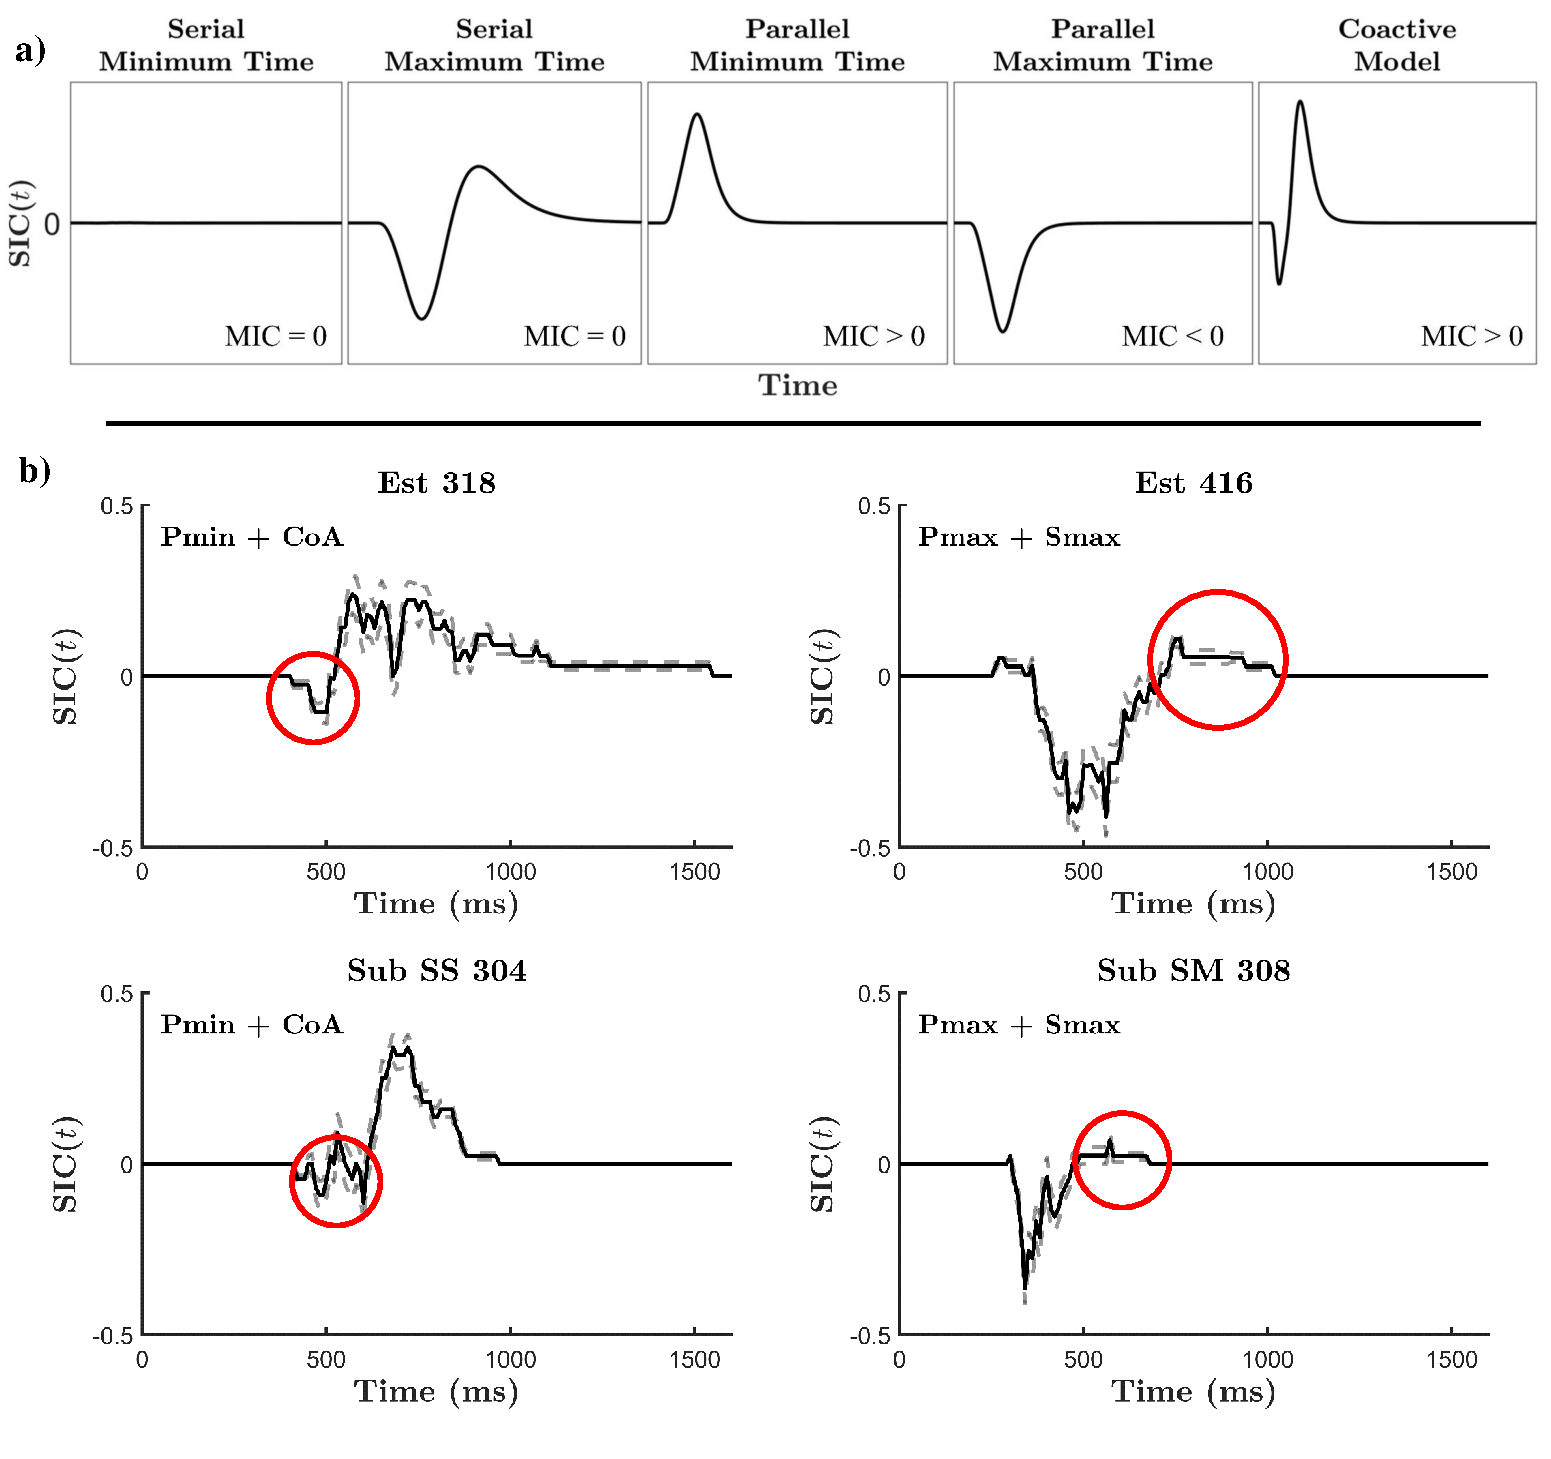
\includegraphics[width=\linewidth]{Figures/Subitizing/MixtureFigure.pdf}
\caption{a. The five canonical SIC functions. b. potential SIC model mixtures from the (top) estimation task, and (bottom) subitizing task. Left: parallel minimum-time models mixed with a coactive model. Right: parallel maximum-time models mixed with a serial exhaustive model. Identifying mixture signatures are circled in red.}
\label{fig:subSICmix}
\end{figure}

Participants Est 416 displays a negative SIC($t$) function, with a late positive deviation. The majority of the SIC($t$) function matches the predictions of a parallel maximum-time processing model; however, the late positive `blip' is indicative of a serial maximum-time model. This signature might suggest that, on a small proportion of trials, processing architecture switched from being parallel maximum-time to serial maximum-time. A similar mixture model is displayed by participant Sub SM 308. 

Visual identification of processing mixture models is rather subjective. Without the ability to identify mixture models through a non-parametric method (à la SFT), previous research has turned to parametric methods of mixture model classification \cite{Little2011, Moneer2016, Cheng2017}. In the following Chapter, we will address this limitation to the SFT machinery. First, we will systematically vary and combine the relative proportions of component processing models and express these mixtures visuallly with our distributional response-time measures. Then, we will extend the tools of SFT and consider a non-parametric method for identifying mixture models. 
\color{black}

\subsection{Conclusion}
Often in life, we need to subitize a set of items, be it coins in our wallet, people in a queue, or discs in a research laboratory\footnote{Admittedly, this is more common for some than others}. Little research has been conducted on how we subitize multiple item-sets, and no research has considered the cognitive architecture or workload capacity, experienced by this system. This is the first known study to address this question, and in so doing, apply the machinery of SFT to subitizing systems. Results of the current study align with findings from within the range of estimation. When asked to subitize two item-sets and decide if either contained less-than a criterion, participants experienced severe limitations to workload capacity. The ubiquity of this finding between participants, and across large and small item-sets, has led us to speculate this might be caused by perceptual context effects. Within the range of subitizing, processing architecture was predominantly serial, yet, select participants displayed patterns consistent with parallel processing architectures. It appears that, while cognitive workload is limited in every individual, processing architecture varies. 

%% AMI DONE 31/10/2019 @@@@@@@@@
